\documentclass{article}
\usepackage[margin=1in]{geometry}
\usepackage{amsmath}
\usepackage{amsthm}
\usepackage{amssymb}
\usepackage{graphicx}

\title{Assignment 3}
\author{Monte Fischer}

\begin{document}

\maketitle

\section*{Problem 1}
For a deterministic policy $\pi_D: \mathcal{S} \to \mathcal{A}$ we have the following equations which follow from replacing terms of the form $\sum \pi(s, a) g(a)$ with $g(\pi_D(s)$ in the nondeterministic MDP Bellman Policy equations.

\begin{align}
    V^{\pi_D}(s) &= Q^{\pi_D}(s, \pi_D(s)) \\
    Q^{\pi_D}(s,a) &= R(s,a) + \gamma \sum_{s^\prime \in \mathcal{S}} P(s,a,s^\prime) V^{\pi_D}(s^\prime) \\
    V^{\pi_D} &= R(s, \pi_D(s)) + \gamma \sum_{s^\prime \in \mathcal{S}} P(s,\pi_D(s),s^\prime)V^{\pi_D}(s^\prime)
\end{align}

\section*{Problem 2}

We will exploit the fact that rewards depend only on action, not on the state. Thus $Q^*(s,a) = Q^*(a)$ and so from the Bellman optimality equation, $V^*(s) = \max_a Q^*(s,a) = \max_a Q^*(a)$ and thus $V^*(s) = V^*(t)$ for any $s,t \in \mathcal{S}$. Then computing,

\begin{align}
    V^*(s) &= \max_a Q^*(s,a)\\
           &= \max_a \{ R(s,a) + \gamma (P(s,a,s)V^*(s) + P(s,a,s+1)V^*(s+1))\}\\
           &= \max_a \{ a(1-a) + (1-a)(1+a) + \frac{1}{2}((1-a)V^*(s) + aV^*(s+1)) \}\\
           &= \max_a \{ 1 + a - 2a^2 + \frac{1}{2} V^*(s)\}
\end{align}
This function of $a$ is maximized at $a = \frac{1}{4}$ by elementary algebra, in which case
\[V^*(s) = 1 + \frac{1}{4} -2\left(\frac{1}{4}\right)^2 + \frac{V^*(s)}{2}\]
and thus
\[ V^*(s) = 2\left(1 + \frac{1}{8}\right) = \frac{9}{4} \quad \forall s \in \mathcal{S}.\]
Incidentally we have also computed an optimal deterministic policy, namely $\pi^D(s) = \frac{1}{4}$ for all $s \in \mathcal{S}$.

\section*{Problem 3}

For code, see the Jupyter notebook \texttt{lilypad.ipynb} in the \texttt{assignment3} directory. We observe from the below graph of optimal escape probability against problem size that a maximum occurs at $n=7$, before which the optimal escape probability is increasing in $n$ and after which the graph is decreasing in $n$.

\begin{figure}[h!]
    \centering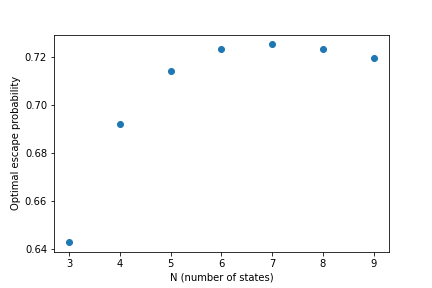
\includegraphics[width=0.8\linewidth]{opt_esc_prob.png}
\end{figure}

\section*{Problem 4}

When $\gamma=0$, the problem reduces to the elementary calculation:
\begin{align}
    \min_a \mathbb{E}_{s^\prime \sim \mathcal{N}(s,\sigma)^2} [e^{as^\prime}] &= \min_a \int_{-\infty}^{\infty} e^{ax} \cdot \frac{1}{\sqrt{2\pi}\sigma} e^{-(x-s)^2 / (2\sigma^2)} dx
\end{align}
This can be solved by computing $a$ such that
\begin{align}
    0 &= \frac{d}{da} \int_{-\infty}^{\infty} e^{ax} \cdot \frac{1}{\sqrt{2\pi}\sigma} e^{-(x-s)^2 / (2\sigma^2)} dx\\
      &= \int_{-\infty}^{\infty} \frac{d}{da} e^{ax} \cdot \frac{1}{\sqrt{2\pi}\sigma} e^{-(x-s)^2 / (2\sigma^2)} dx\\
      &= e^{as + a^2 \sigma^2 /2}(s+a\sigma^2)
\end{align}
and thus
\begin{equation}
    a = -\frac{s}{\sigma^2} 
\end{equation}
attains the minimum expected myopic cost at for any state $s$. Substituting this back into the above expectation, we see with a little calculation that the optimal expected cost is $\frac{1}{\sqrt{2}}$ for all $s$.

\end{document}
